\begin{figure}[t]
\centering
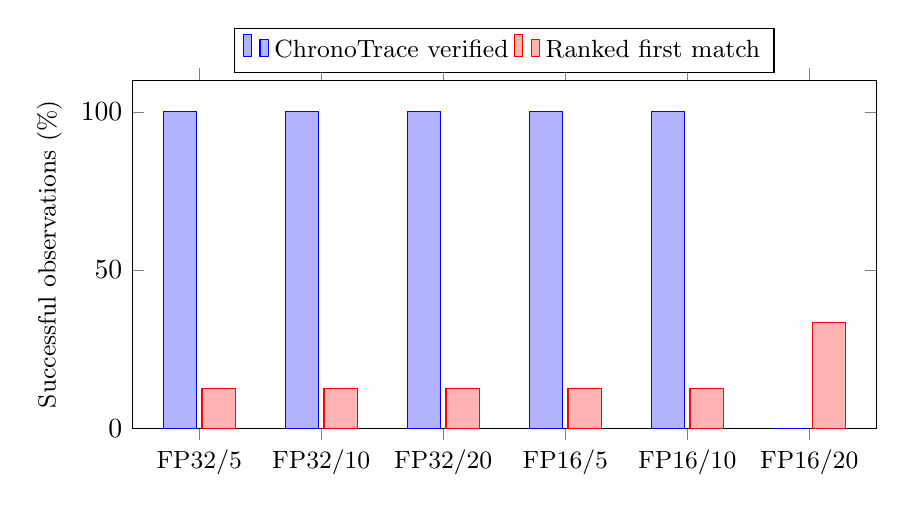
\begin{tikzpicture}
\begin{axis}[width=.91\linewidth,height=6.0cm,ybar,bar width=12pt,
 ymin=0,ymax=110,ylabel={Successful observations (\%)},
 symbolic x coords={32/5,32/10,32/20,16/5,16/10,16/20},xtick=data,
 xticklabels={FP32/5,FP32/10,FP32/20,FP16/5,FP16/10,FP16/20},
 x tick label style={font=\small},ylabel style={font=\small},
 legend style={at={(.5,1.02)},anchor=south,legend columns=2,font=\small},
 enlarge x limits=.11]
\addplot coordinates {(32/5,100)(32/10,100)(32/20,100)(16/5,100)(16/10,100)(16/20,0)};
\addplot coordinates {(32/5,12.5)(32/10,12.5)(32/20,12.5)(16/5,12.5)(16/10,12.5)(16/20,33.3333)};
\legend{ChronoTrace verified,Ranked first match}
\end{axis}
\end{tikzpicture}
\caption{Coverage by export format and stage duration at matched gradient-work budgets (24 observations per cell). Verification and first-match retrieval are different outputs. The strong-FP16 reversal is retained. Training and replay remain FP64 throughout.}
\label{fig:coverage}
\end{figure}
